\section{Attacking Property-preserving Encryption}

\subsection{Number of unique first names in the database}

In the database are stored 100 unique first names. This number was determined by taking into consideration that the names in the database were encrypted using deterministic encryption. As a consequence, the number of unique encripted first names is equivalent to the number of first names in the database.

\begin{lstlisting}[language = Java, caption=Java Code to Count Unique First Names, firstnumber = last , escapeinside={(*@}{@*)}]
    public int getFirstNameCount() {
        String query = "SELECT COUNT(DISTINCT enc_firstname) FROM enc_students";
    
        try (Connection conn = DriverManager.getConnection(url);
             PreparedStatement pstmt = conn.prepareStatement(query);
             ResultSet rs = pstmt.executeQuery()) {
    
            if (rs.next()) {
                return rs.getInt(1);
            }
    
        } catch (SQLException e) {
            System.out.println("Error: " + e.getMessage());
        }
        return 0;
    }
\end{lstlisting}

\subsection{Distribution of last names}

Following, the code to compute the lastname frequency.

\begin{lstlisting}[language = Java, caption = Distribution of last names, firstnumber = last , escapeinside={(*@}{@*)}]

    public HashMap<String, Integer> getLastnameFrequenciesOrdered() {
        String query = "SELECT enc_lastname FROM enc_students";

        try (Connection conn = DriverManager.getConnection(url);
             PreparedStatement pstmt = conn.prepareStatement(query);
             ResultSet rs = pstmt.executeQuery()) {

            HashMap<String, Integer> lastnameFrequencies = new HashMap<>();
            while (rs.next()) {
                String lastname = rs.getString("enc_lastname");
                if (lastnameFrequencies.containsKey(lastname)) {
                    lastnameFrequencies.put(lastname, lastnameFrequencies.get(lastname) + 1);
                } else {
                    lastnameFrequencies.put(lastname, 1);
                }
            }
            
            return orderHashMapByValue(lastnameFrequencies);

        } catch (SQLException e) {
            System.out.println("Error: " + e.getMessage());
        }
        return null;
    }
\end{lstlisting}

Following, the graph with lastnames in chipertext.

\begin{figure}[h!]
    \centering
    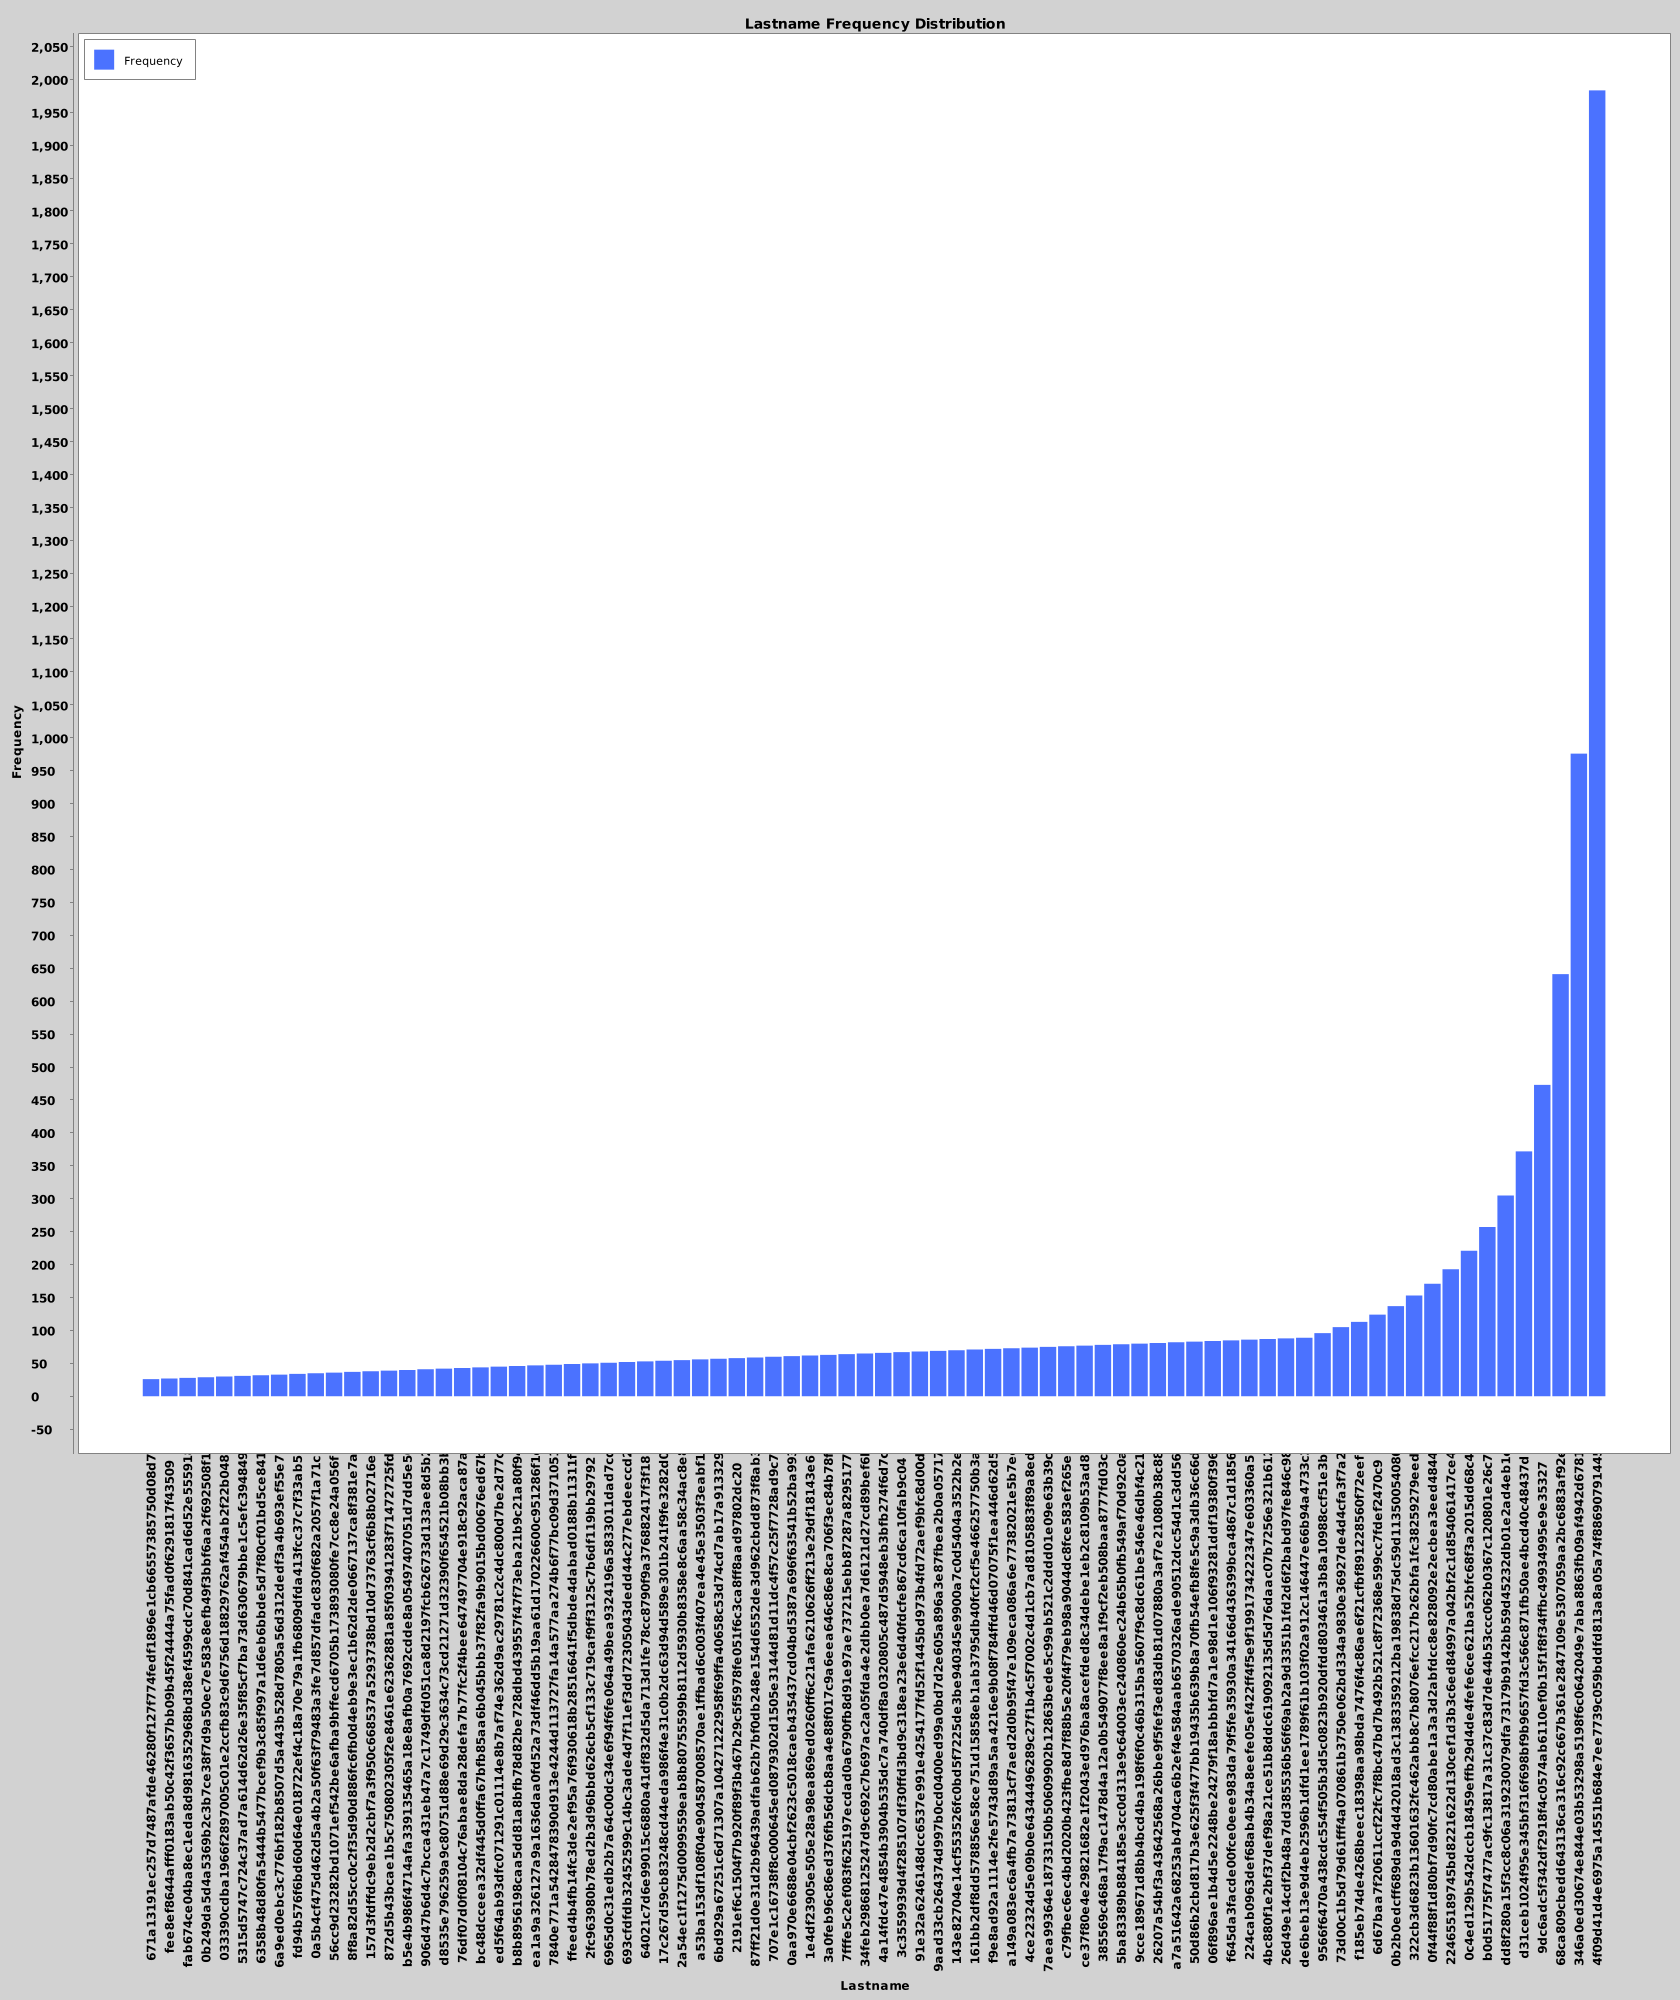
\includegraphics[width=\textwidth]{03-ex2/Lastname_Frequency_Distribution.png}
    \caption{Distribution of encrypted last names.}
    \label{fig:Distribution-of-last-names}
\end{figure}

The graph shows the distribution of the encrypted last names last names. The distribution is clearly non-uniform, and an attacker can use background information (like the files given for this assignment) to infer craft a lookup table for mapping encrypted values to plaintext values.

Following, the same graph with names in plaintext.

\begin{figure}[h!]
    \centering
    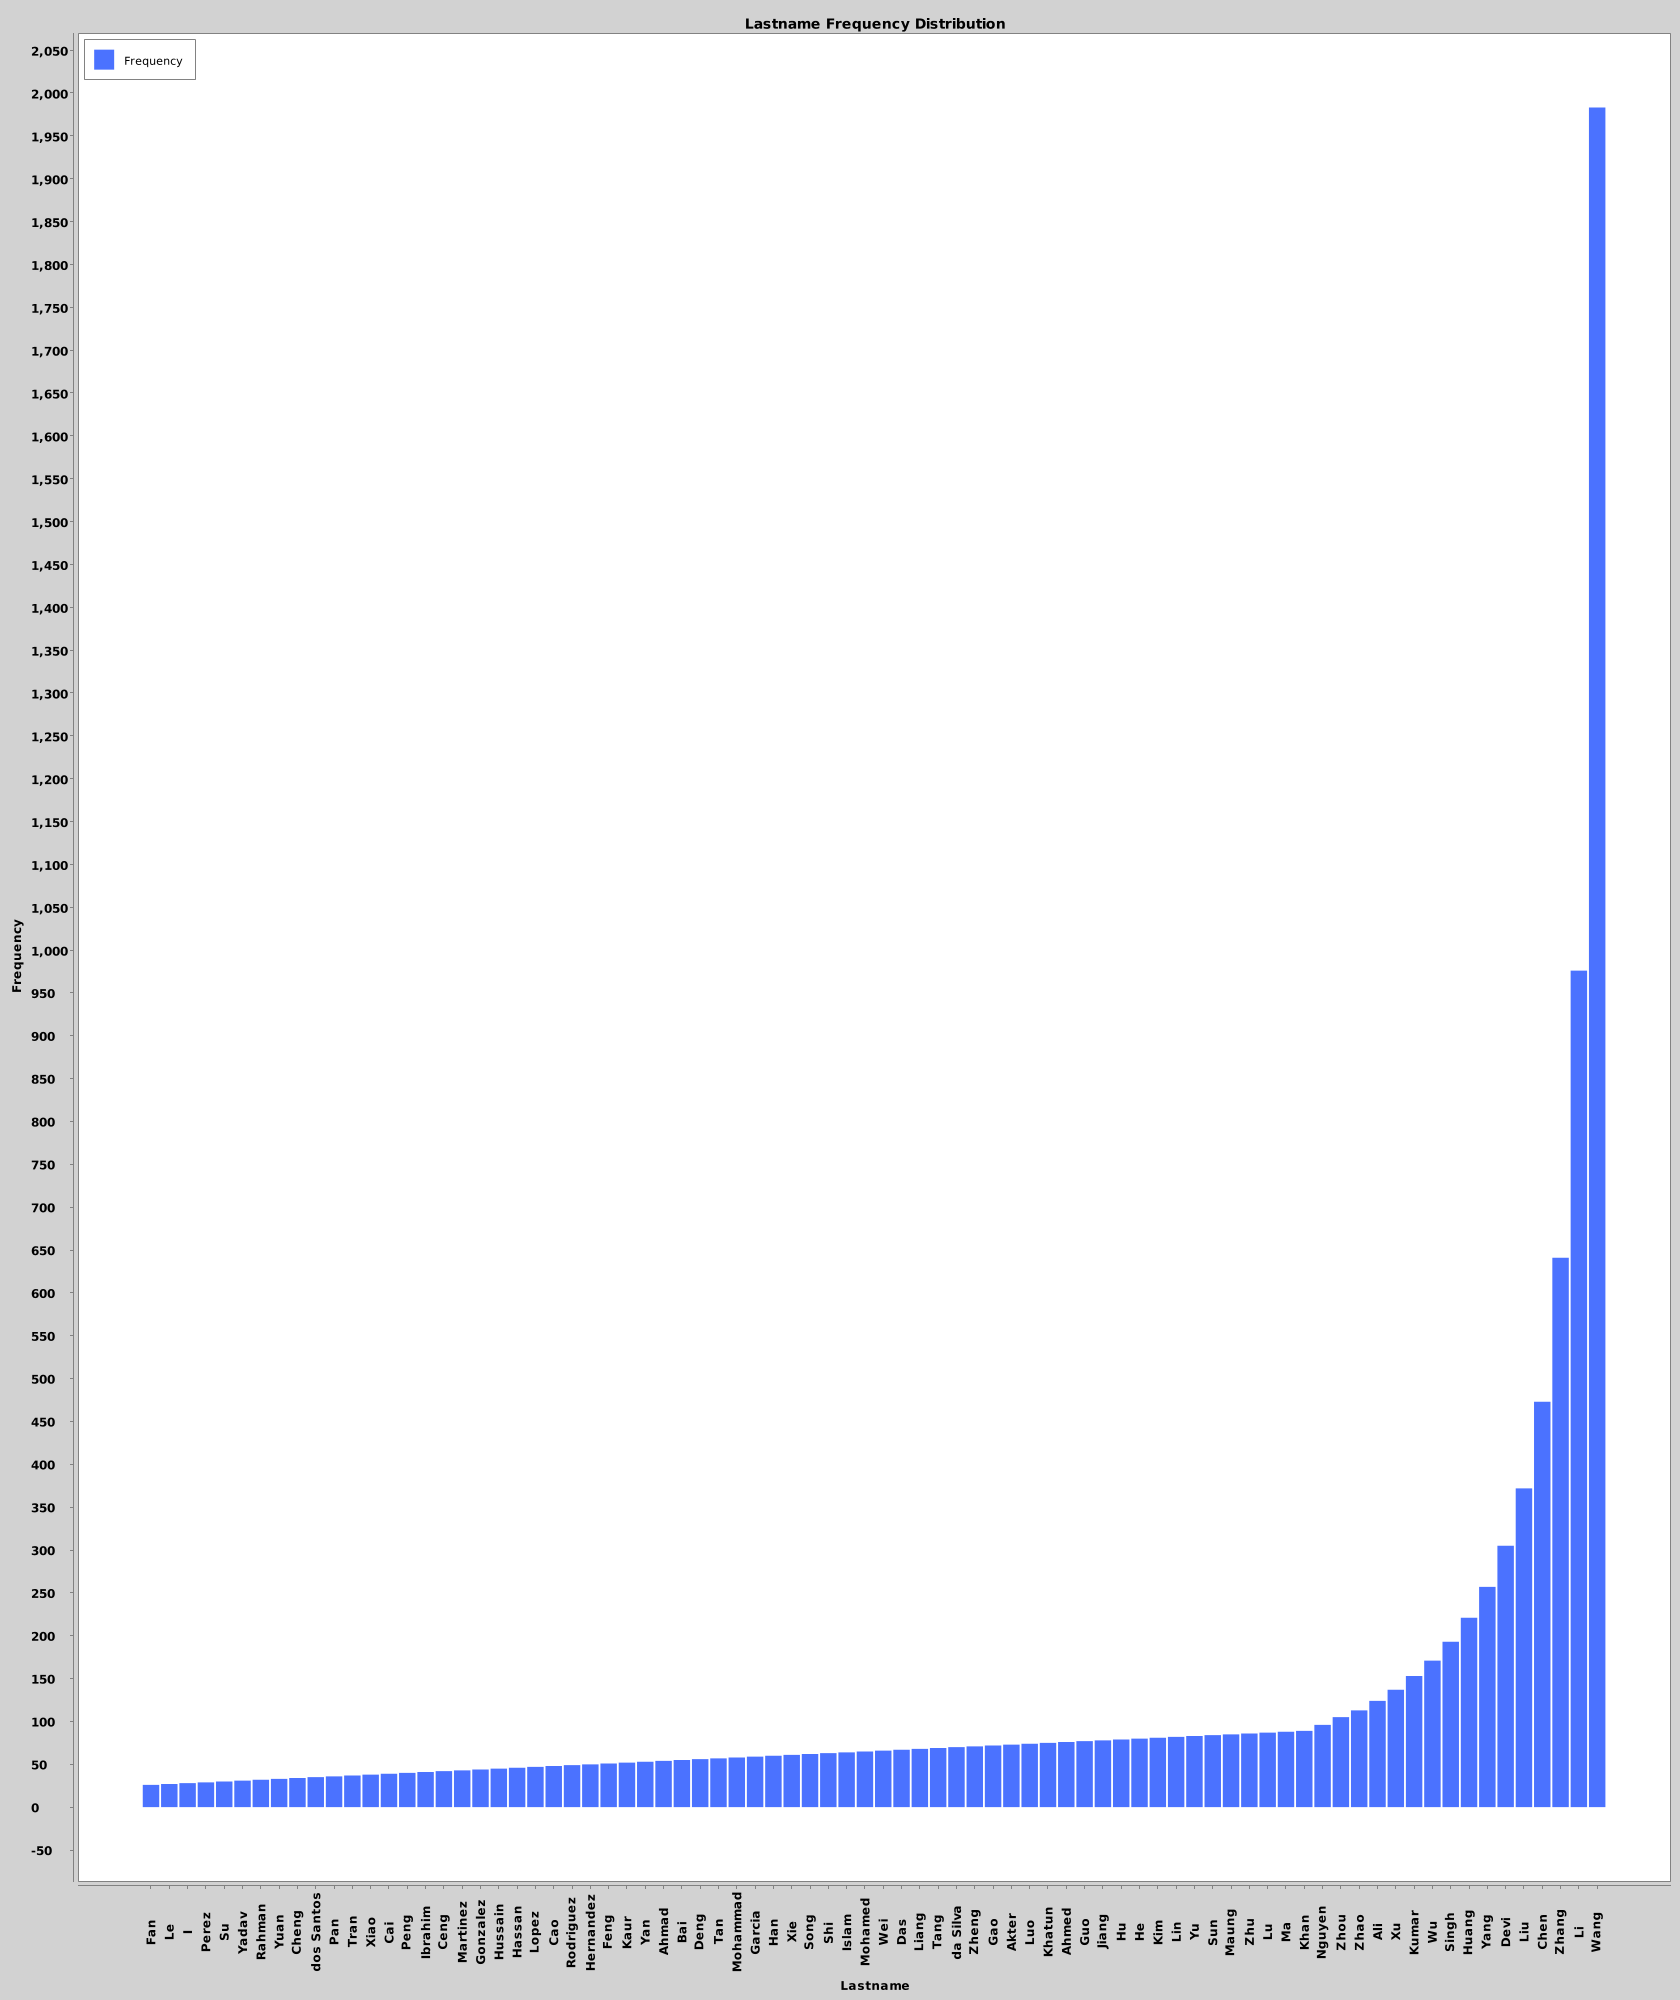
\includegraphics[width=\textwidth]{03-ex2/Lastname_Frequency_Distribution_Plain.png}
    \caption{Distribution of encrypted last names.}
    \label{fig:Distribution-of-last-names-plain}
\end{figure}

As can be seen, lastname Wang is mapped to chipertext \\ \texttt{4f09d41d4e6975a14551b684e7ee7739c059bddfd813a8a05a74f88690791445}.

\subsection{Full names of all students who scored 99 points}

\begin{lstlisting}[language = Java, caption = Querying for the students who got 99, firstnumber = last , escapeinside={(*@}{@*)}]
public String getSecondUniqueHighestValue() {
        String query = "SELECT enc_grade FROM ("
                + "    SELECT DISTINCT enc_grade"
                + "    FROM enc_students"
                + "    ORDER BY enc_grade DESC"
                + ") as eseg LIMIT 1 OFFSET 1;";

        try (Connection conn = DriverManager.getConnection(url);
             PreparedStatement pstmt = conn.prepareStatement(query)) {

            // Execute the query
            ResultSet rs = pstmt.executeQuery();

            // Process the result
            if (rs.next()) {
                return rs.getString("enc_grade");
            }
        } catch (SQLException e) {
            System.out.println(e.getMessage());
        }
        return null;
    }

    public List<Student> getSecondToTopStudents() {
        String secondValue = getSecondUniqueHighestValue();
        String query = "SELECT enc_firstname, enc_lastname FROM enc_students WHERE enc_grade = ?";
        List<Student> resultList = new ArrayList<>();

        try (Connection conn = DriverManager.getConnection(url);
             PreparedStatement pstmt = conn.prepareStatement(query)) {

            pstmt.setString(1, secondValue);
            ResultSet rs = pstmt.executeQuery();

            ResultSetMetaData metaData = rs.getMetaData();
            int columnCount = metaData.getColumnCount();

            while (rs.next()) {
                Student student = null;
                for (int i = 1; i <= columnCount; i++) {
                    student = new Student(
                            rs.getString("enc_firstname"),
                            secondValue,
                            rs.getString("enc_lastname")
                    );
                }
                resultList.add(student);
            }

        } catch (SQLException e) {
            System.out.println("Error: " + e.getMessage());
        }

        return resultList;
    }
\end{lstlisting}

\subsection{Implementing $(\alpha, t)$-secure index as mitigation}

Following, the graph of lastnames' frequencies after implementing a $(4, 0)$-secure index search.

\begin{figure}[h!]
    \centering
    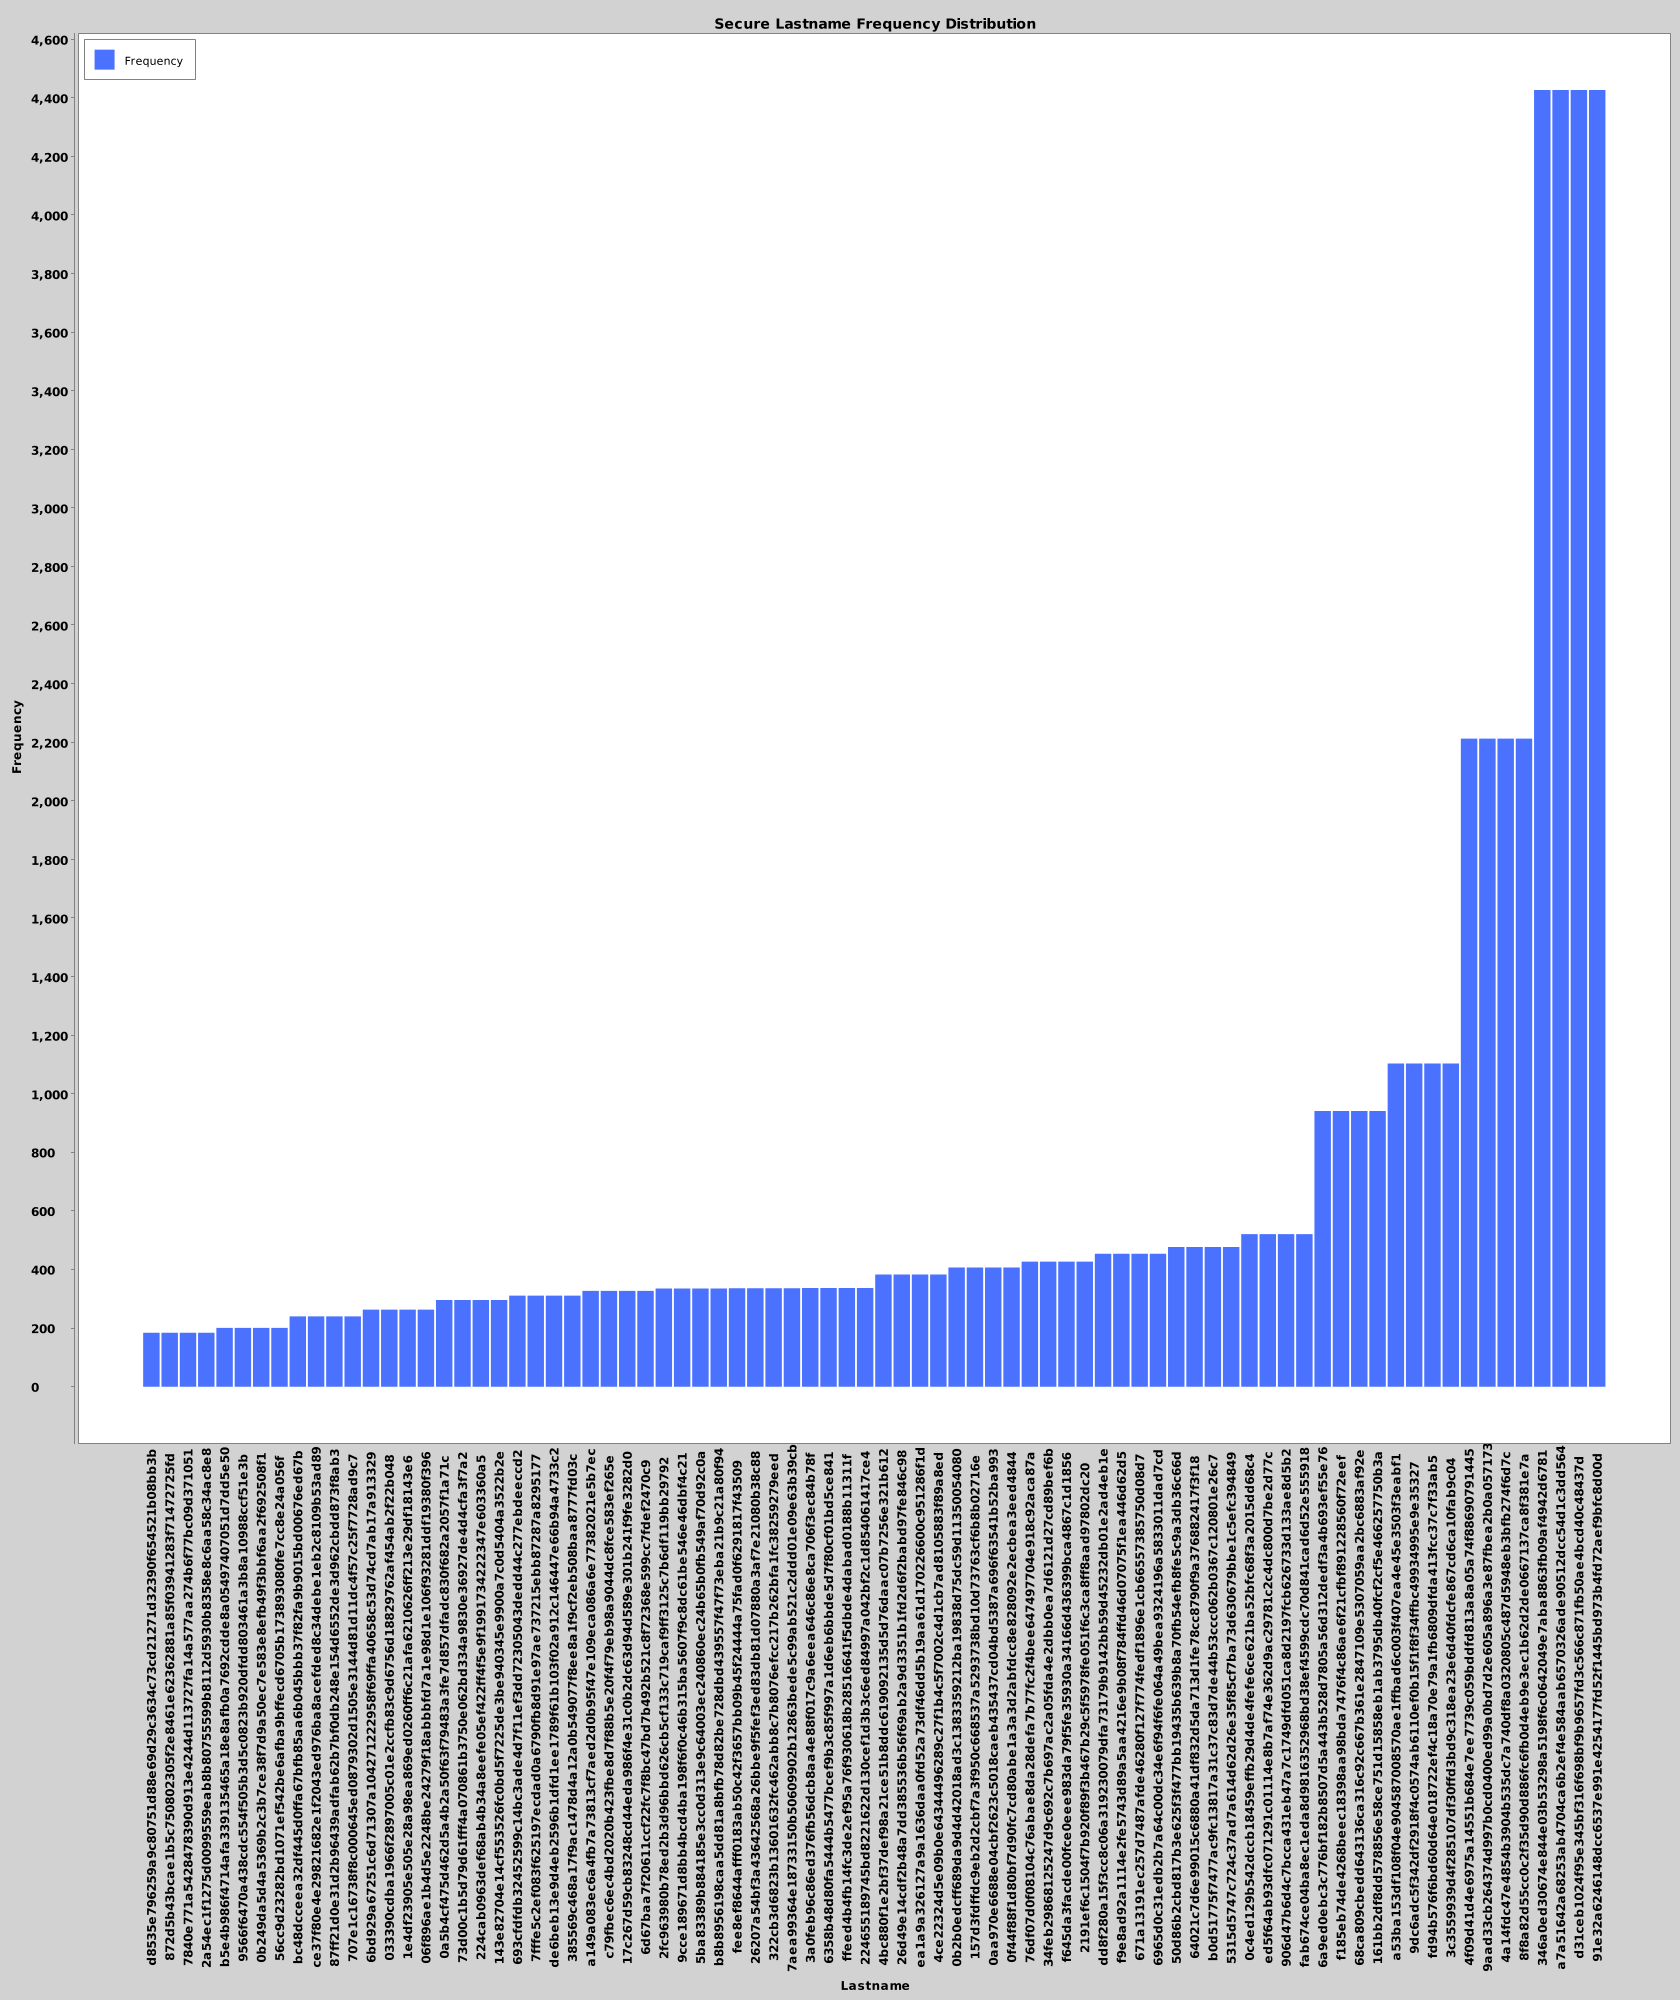
\includegraphics[width=\textwidth]{03-ex2/Secure_Lastname_Frequency_Distribution.png}
    \caption{Distribution of encrypted last names.}
    \label{fig:Distribution-of-last-names-sec}
\end{figure}

The graph shows the distribution of the encrypted last names last names. The distribution is clearly non-uniform, and an attacker can use background information (like the files given for this assignment) to infer craft a lookup table for mapping encrypted values to plaintext values.

Following, the same graph with names in plaintext.

\begin{figure}[h!]
    \centering
    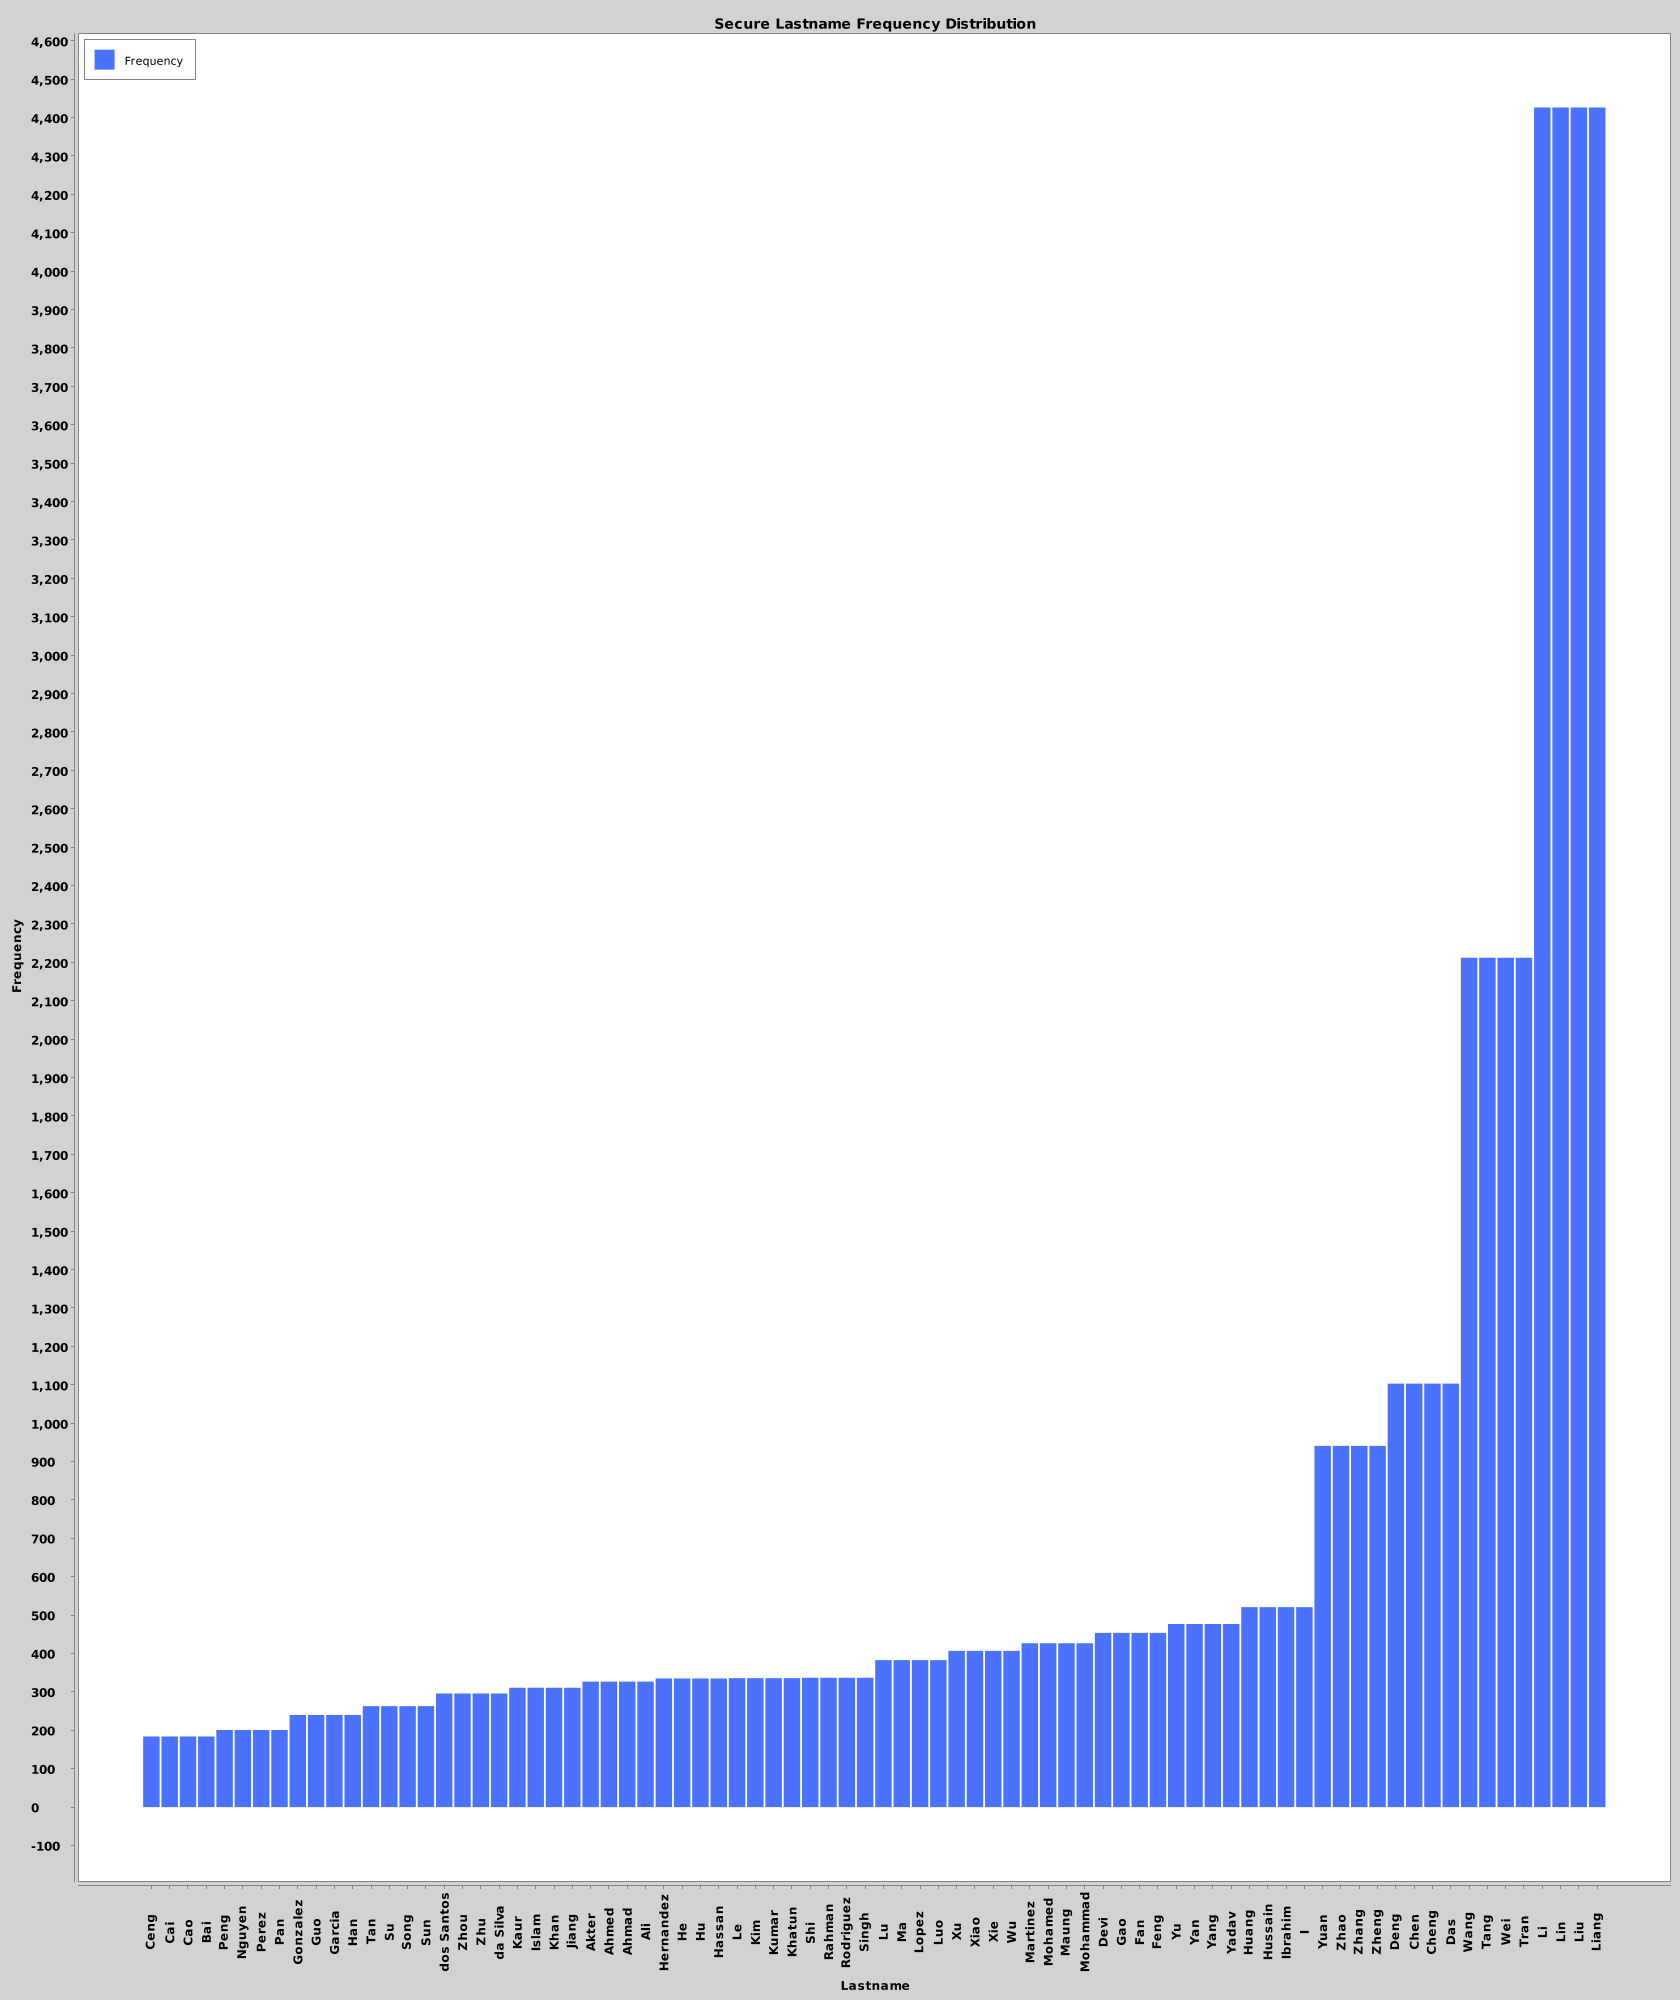
\includegraphics[width=\textwidth]{03-ex2/Secure_Lastname_Frequency_Distribution_Plain.png}
    \caption{Distribution of encrypted last names.}
    \label{fig:Distribution-of-last-names-plain-sec}
\end{figure}

Following, the code 

\begin{lstlisting}[language = Java, caption = secure index as mitigation, firstnumber = last , escapeinside={(*@}{@*)}]

    public List<Student> getSecStudentsFromSurname(String surname, int alpha) {
        List<Student> students = new java.util.ArrayList<>();
        int i = surnameList.indexOf(surname);

        //compute cluster boundaries
        int clusterUpperBound = i;
        for (int j = i; (j % alpha != 0 || j==i) && (j<rows); j++) {
            clusterUpperBound = j;
        }
        int clusterLowerBound = i;
        for (int j = i; (j % alpha != 0) && j>0 ; j--) {
            clusterLowerBound = j-1;
        }

        //return students in alpha-size cluster
        if(i != -1) {
            for (int j = i; j <= clusterUpperBound && (j<rows); j++) {
                for (int k = 0; k < cols; k++) {
                    if (matrix[j][k]) {
                        students.add(studentList.get(k));
                    }
                }
            }
            i--;
            for (int j = i; j >= clusterLowerBound; j--) {
                for (int k = 0; k < cols; k++) {
                    if (matrix[j][k]) {
                        students.add(studentList.get(k));
                    }
                }
            }
        }

        return students;
    }
\end{lstlisting}